\documentclass[11pt]{article}
\usepackage{amsmath}
\usepackage{fontspec}
\setmainfont[Mapping=tex-text]{MS Mincho}
\XeTeXlinebreaklocale "ja"
\XeTeXlinebreakskip=0pt plus 1pt
\XeTeXlinebreakpenalty=0
\usepackage{graphicx}
\usepackage[margin=0.5in]{geometry}
\setlength{\parindent}{0cm}

\begin{document}

膝の曲がり具合によって(角度$\alpha$)足全体の慣性モーメントがどう変化するかを調べる。

足の付け根を軸にしたときの足の慣性モーメントは次のように定義される:

$$ \Gamma = \iiint_V r^2 dV $$

足を体位長さあたりの重量 $\rho$ の線状のものにモデル化する。
足の付け根から膝までの長さを $L$ とした上で、膝から足首までの長さもそれと同一視し $=L$ とする。 足首より下の部分の重さを無視する。

\begin{figure}[h!]
\centering
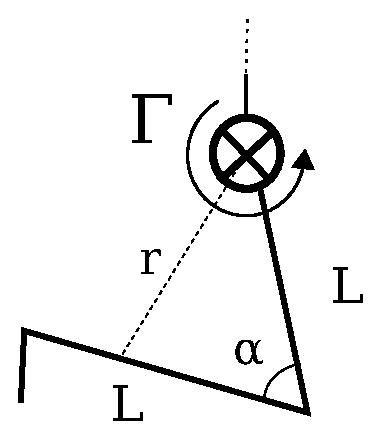
\includegraphics[width=0.12\textwidth]{leg_model.eps}
\end{figure}
慣性モーメントは次の形になる:

\begin{equation}
\begin{split}
\Gamma & \simeq \rho\int_0^L l^2 dl + \rho\int_0^L (L - l\cos\alpha)^2 + (l\sin\alpha)^2 dl\\
 & = \rho\left[l^3/3\right]_0^L + \rho\int_0^L (L^2 + l^2\cos^2\alpha - 2Ll\cos\alpha + l^2\sin^2\alpha) dl\\
 & = \rho L^3/3 + \int_0^L (L^2 + l^2 - 2Ll\cos\alpha) dl\\
 & = \rho L^3/3 + \rho\left(L^2\left[l\right]_0^L + \left[l^3/3\right]_0^L - 2L\cos\alpha\left[l^2/2\right]_0^L \right)\\
 & = \rho L^3/3 + \rho L^3\left(4/3 - \cos\alpha  \right)
\end{split}
\end{equation}

以下は$\Gamma'=\Gamma/\rho{}L$の正規化された慣性モーメントのグラフを示す。

\begin{figure}[h!]
\centering
\includegraphics[width=0.6\textwidth]{plot.eps}
\end{figure}

\end{document}